\chapter{\label{ch:detector} The Compact Muon Spectrometer detector}	
  The Compact Muon Spectrometer (CMS) is housed at interaction point 5 of the 
    LHC. 
  The LHC is designed to pursue physics at the TeV scale. 
  This is the scale where electroweak symmetry breaking is believed to occur
  	\cite{CmsPTdrv2}.
  While this means that the search for the standard model Higgs boson was the 
    central driving design consideration, the wide range of possibilities for
  	finding new physics signals requires a general purpose detector.
  The expedient discovery of new physics through low cross section interactions 
  	requires high luminosity.
  Muon capabilities developed for the Higgs boson can be used to study \JPsi{}. 
  A versatile trigger is needed to accommodate the high interaction rates that 
    accompany the high luminosities. 
  By exploiting the versatility of the trigger and muon systems it
    is possible to explore processes like UPC \JPsi{} production, 
    which push to the low energy edge of the experiment's capabilities. 
  \begin{figure}[h]
    \centering
      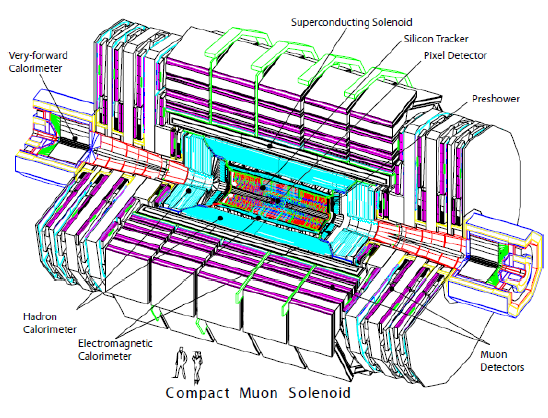
\includegraphics[width=.5\textwidth]{cms}
    \caption{The Compact Muon Solenoid layout \cite{tCmsE}.}
    \label{cms}
  \end{figure}
  
  The general purpose design of CMS is dominated by the massive 4T 
  	superconducting solenoid at its core.
  The magnets is 13m long with a 6m diameter, and pushes the limits of power
  	and compactness \cite{tCmsE}. 
  These two conflicting limits are achieved through the novel design of 
  	interweaving structural and conducting elements together in the coil of
  	the solenoid.

  Within the solenoid resides three different sub detectors.
  The inner most is the world's largest silicon tracker \cite{tCmsE}.
  The tracker is surrounded by a highly effective lead tungstate crystal 
    electromagnetic calorimeter (ECAL).
  ECAL is encapsulated in a brass scintillating hadronic calorimeter (HCAL).
  Outside the magnet, muon chambers are used to aid in the measurement and 
    triggering of muon events. 
  Altogether CMS weighs 12,500 metric tons, has a diameter of 14.6m,
    and a length of 21.6m \cite{tCmsE}.

  \section{Tracker}
    The Silicon Tracker is the innermost sub-detector of CMS, and has active
    	elements as close as 4.4cm to the interaction point \cite{tCmsE}. 
    The tracker has a length 5.8m, a diameter of 2.6m and
    	covers a range in pseudorapidity of $|\eta| <$ 2.5.
    At the center of the tracker are three rings of silicon pixels around the beam 
    	with two disks of silicon pixels to cap the rings.
    The pixel portion of the silicon tracker is comprised of 66$\times$10$^{6}$
    	pixels.
    The silicon pixels are surrounded by silicon strips.
    The silicon strips are separated into 4 different sections: 
    	the Tracker Inner Barrel, the Tracker Inner Disk, the Tracker Outer 
    	Barrel, and the Tracker End Caps.
    The silicon strip detectors as a whole are comprised of 9.3$\times$10$^{6}$ silicon 
    	strips.
    The high number of pixels and strips allow for the ability to distinguish
    	and collect enough distinct points to reconstruct the path of the 1000
    	or so charged particles per bunch crossing expected at peak luminosity
    	\cite{tCmsE}.
    \begin{figure}[!Hhbt]
      \centering
      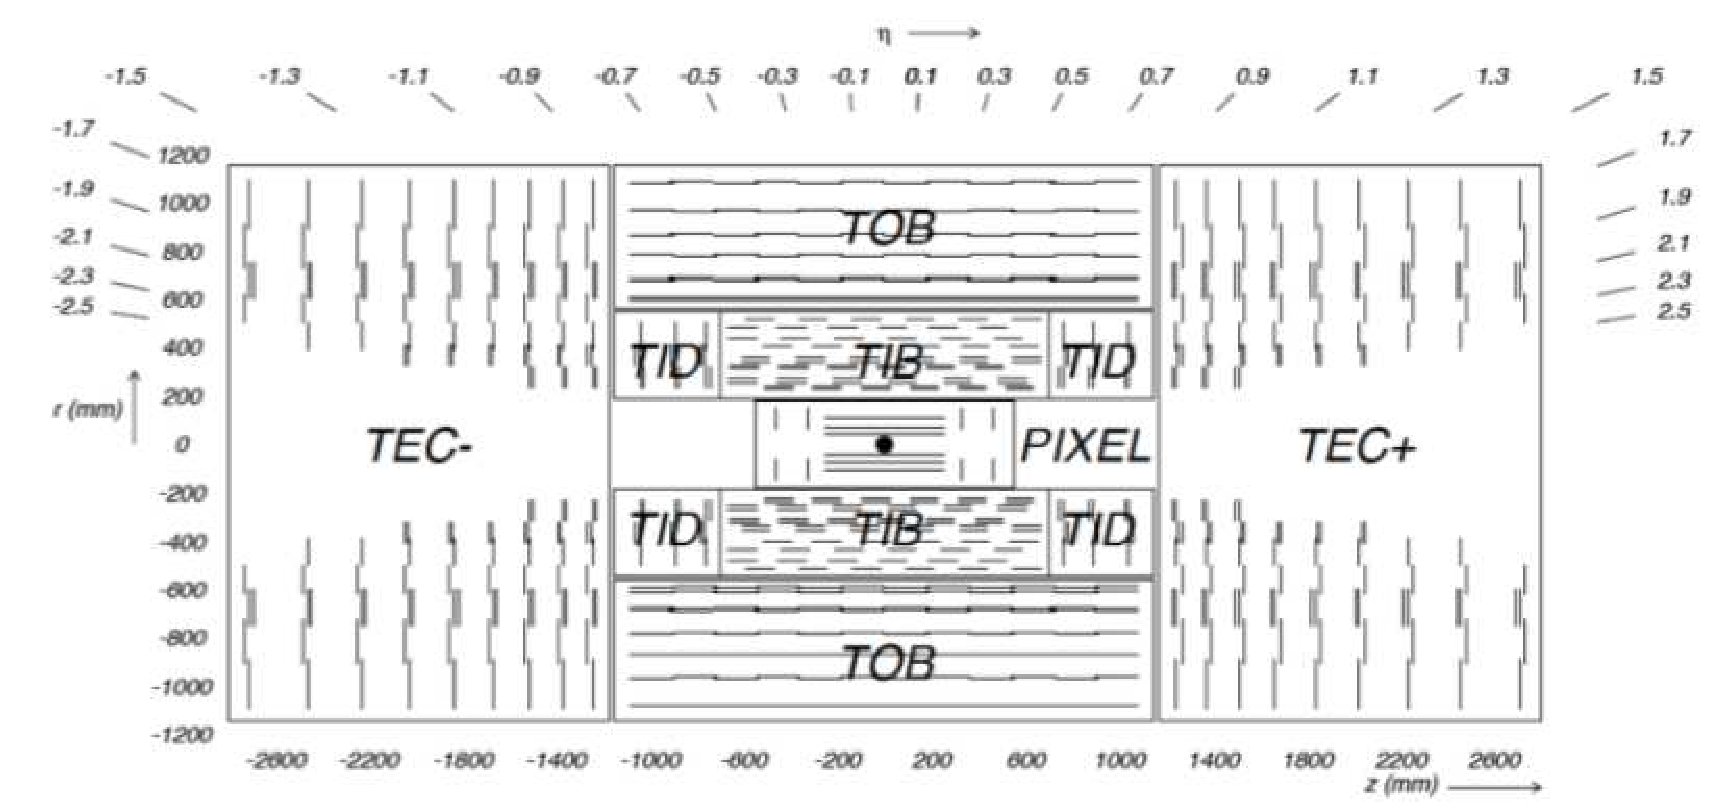
\includegraphics[width=0.75\textwidth]{trackerLayout}
      \caption{Layout of the silicon tracker with the pixels closest to the 
        interaction point, marked with a black dot, and the strips segments 
        beyond the pixels.}
      \label{fig:fig:trackerLayout}
    \end{figure}

    The amount of material present in the tracker is substantial enough to
      alter the path of particles as they pass through the tracker. 
    Fig.~\ref{fig:matBudge} shows the amount of material in the tracker 
      as a function of radiation lengths ($X_{0}$).
    The radiation length is the mean distance a high energy particle travels 
      before giving up one $e$-fold of kinetic energy through electromagnetic
    	interactions.
    For example, after one radiation length $E \rightarrow E/e$, where 
    	$e \sim 2.7$ the base of the natural logarithm. 
    As opposed to the deflection angle set by the strength of the magnetic 
      field, the momentum resolution for lower momentum tracks is limited by 
      the lose of energy due to scattering of these particles off the material 
      of the detector.
    For UPC \JPsi{}, this is the primary factor contributing to the resolution 
      of the reconstructed muon tracks. 
    \begin{figure}[!Hhbt]
      \centering
      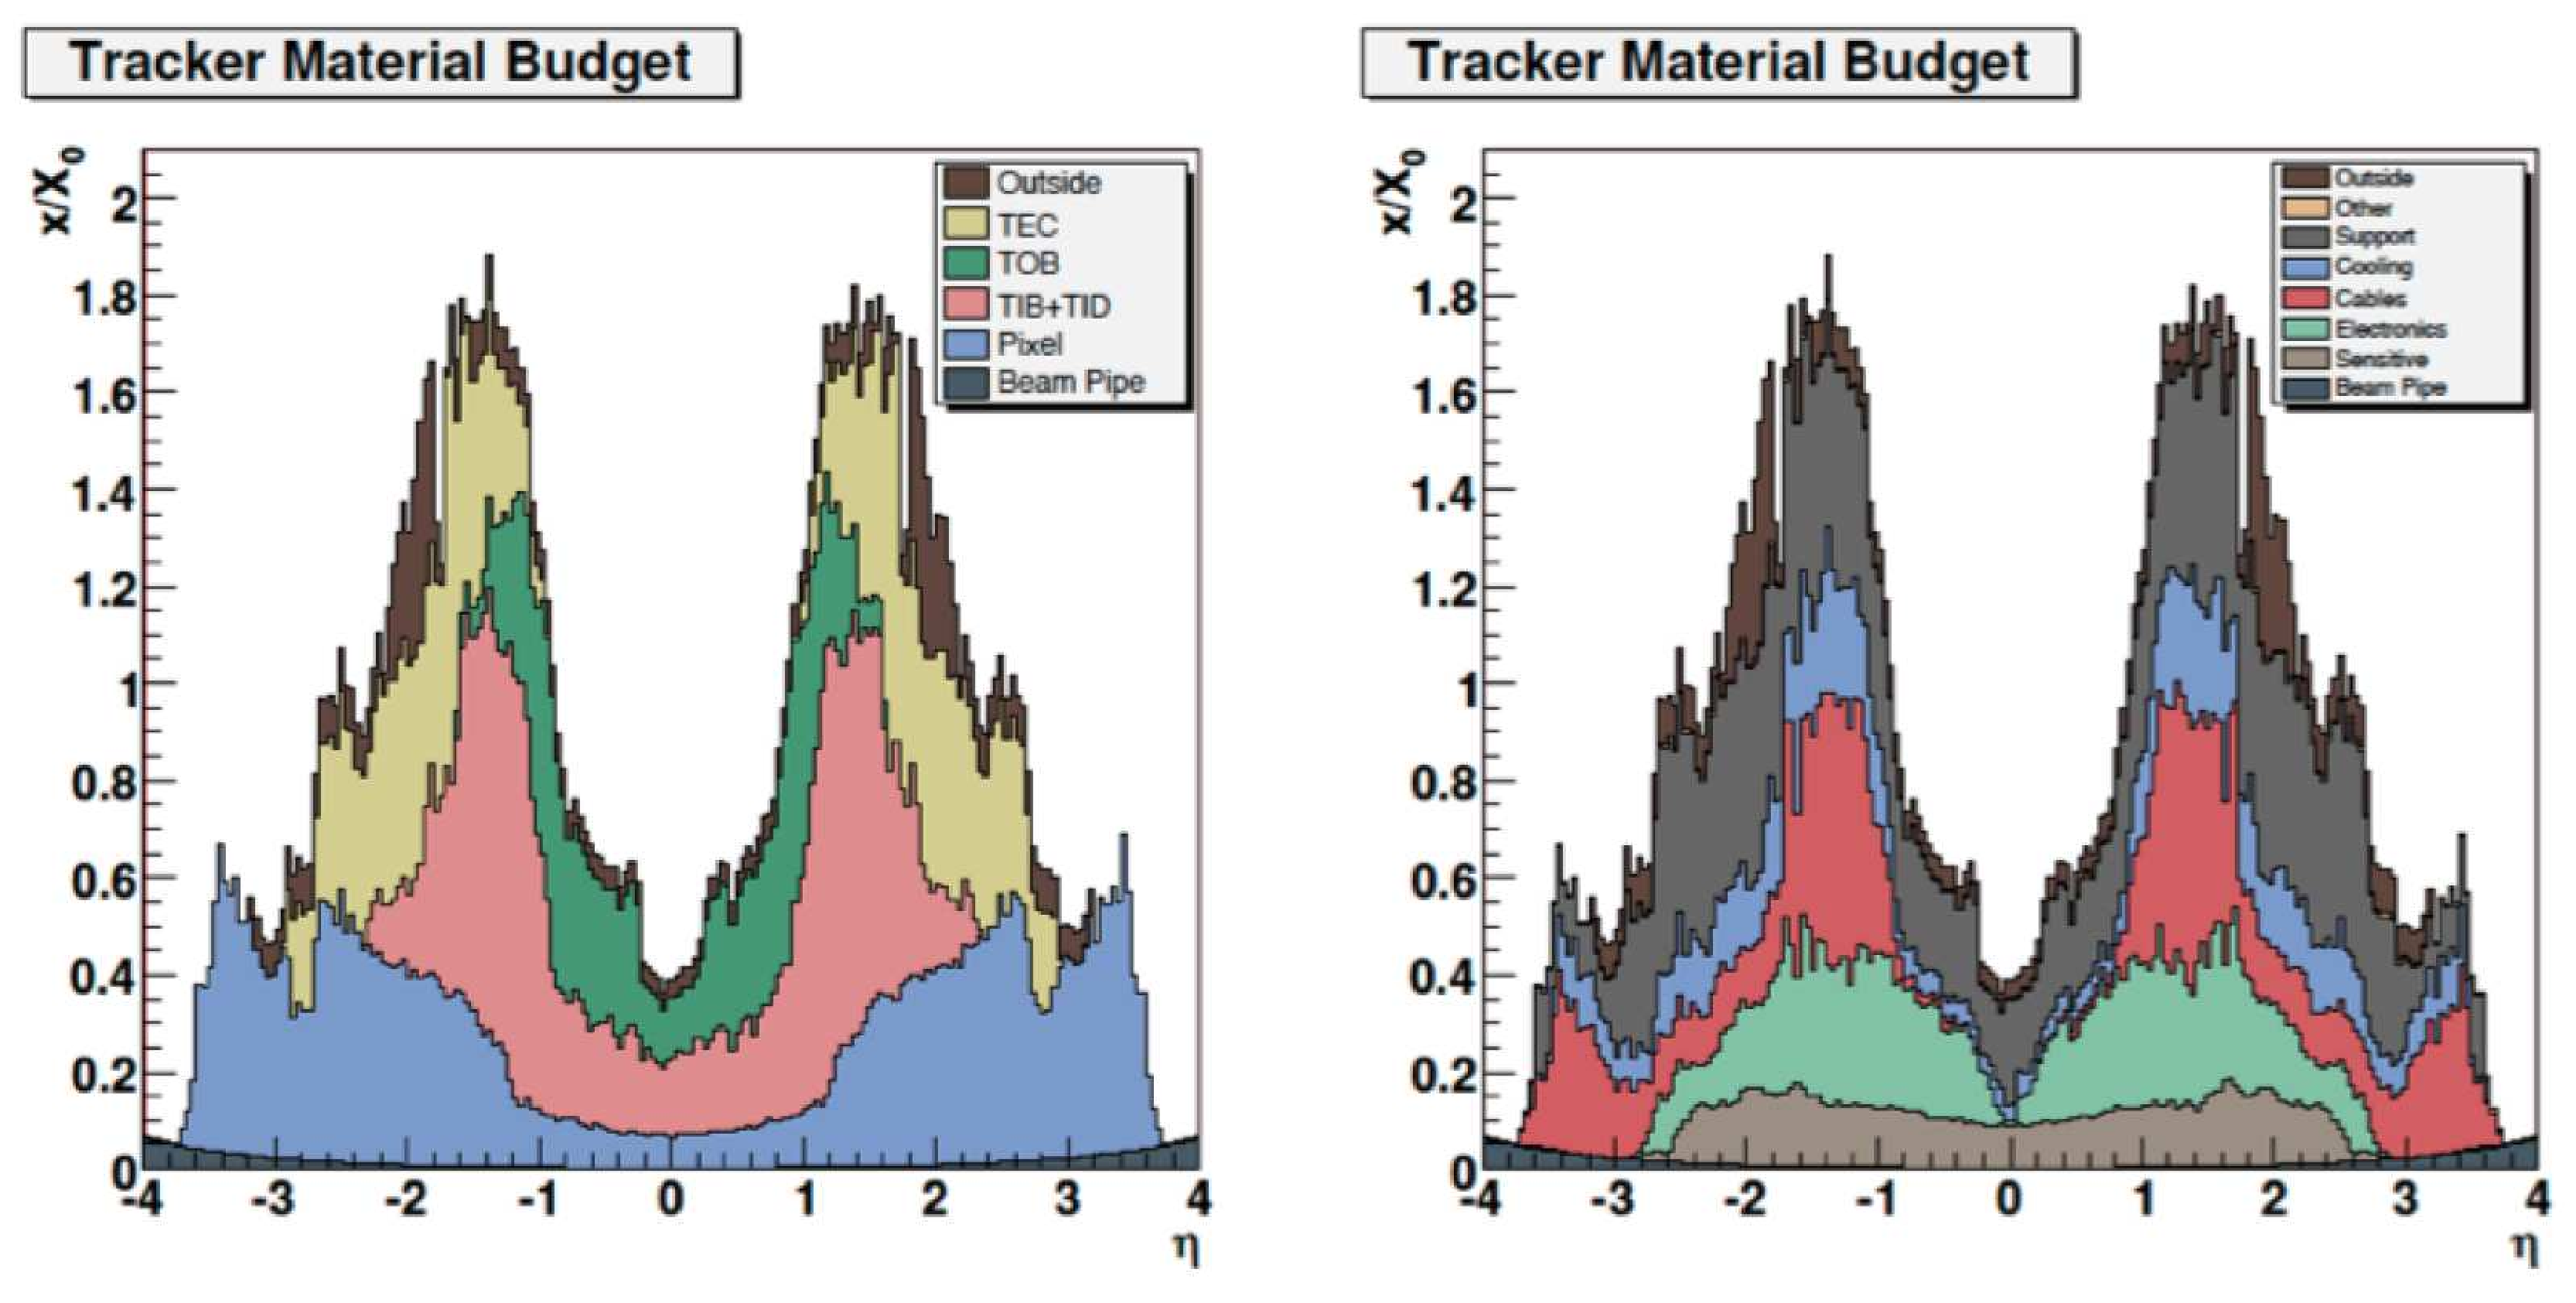
\includegraphics[width=0.65\textwidth]{matBudge}
      \caption{Material budget in the tracker broken down by sub-detector(left) and
        category (right).}
      \label{fig:matBudge}
    \end{figure}

  \section{ECAL}
    The next detector beyond the tracker is the electromagnetic calorimeter 
      system, ECAL.
    The calorimeter system is made of 61,200 lead tungstate (PbWO$_{4}$) 
      crystals in the central barrel and 7,324 on each of the two endcaps 
      \cite{tCmsE}.
    The barrel (EB) covers a pseudorapidity range $|\eta| < 1.479$ and has an
    	$\eta-\phi$ segmentation of approximately $0.0174\times0.0174$, depending
      slightly on the position of the fixed sized crystals.
    Lead tungstate is very dense giving the ECAL crystals a high number of 
      interaction lengths within a short depth.
    The crystals of the barrel have a depth of 230 mm corresponding to 25.8 
    	$X_{0}$.
    The endcaps (EE) cover the pseudorapitity region $1.479 < |\eta| < 3$.
    In the endcap the crystals have an exposed area of 28.62 $\times$ 28.62 
    	mm$^{2}$, and a depth of 220 mm corresponding to 24.7 $X_{0}$.
    The energy resolution of the ECAL as measured by test beam data can be seen in
    	Figure~\ref{ECALeRes}.
    \begin{figure}[!Hhbt]
      \centering
        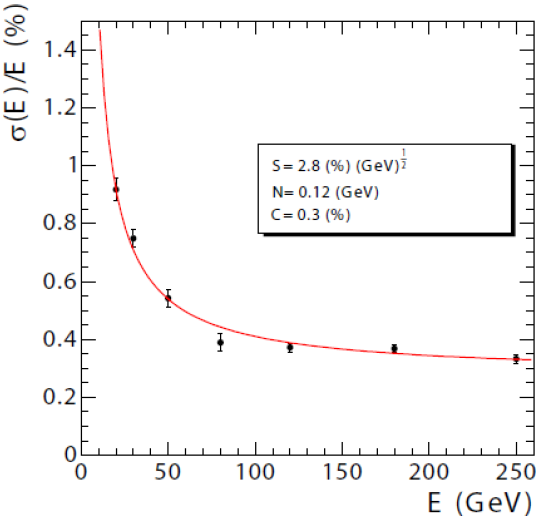
\includegraphics[width=0.5\textwidth]{ECALeRes}
      \caption{The energy resolution of ECAL as a function of energy ~\cite{tCmsE}.}
      \label{ECALeRes}
    \end{figure}
    The fractional energy resolution reduces quickly above 10 GeV and levels
      off at about 0.5\% for energies above 100 GeV. 
    For \JPsi{} with rapidity near 2, the electron will carry at least 10 GeV
      and can be resolved by the ECAL. 

  \section{HCAL}
    The HCAL like the ECAL has both a barrel (HB) and endcaps (HE).
    The pseudorapidity region $|\eta|<1.3$ is covered by HB \cite{tCmsE}. 
    HB has an $\eta-\phi$ segmentation of $0.0897\times0.0897$, and is 25 times more
    	sparsely granulated than EB.
    HE covers the pseudorapidity region $1.3<|\eta|<3$.
    HE, like EE and the tracker endcaps, is aligned perpendicular to the beam axis
    	resulting in granularity that changes with $\eta$.
    In the region $1.3 <|\eta|< 1.6$ HE has an $\eta-\phi$ segmentation of 
    	$0.0897\times0.0897$.
    The $\eta-\phi$ segmentation roughly doubles to $0.17\times0.17$ in the region
    	$1.6 <|\eta|< 3$.
    The energy resolution of the barrel and endcaps can be seen in  
    	Figure~\ref{HCALeRes}.
    The thickness of the hadronic calorimeter is best described in interaction
    	lengths, the mean distance for a particle to give up an $e$-fold of energy
    	through nuclear interactions. 
    At $\eta = 0$ the barrel has a thickness 5.82 interaction lengths 
    	($\lambda_{I}$), and increases as the path length through the material 
    	increases to 10.6 $\lambda_{I}$ at $|\eta| = 1.3$.
    \begin{figure}[h]
      \centering
        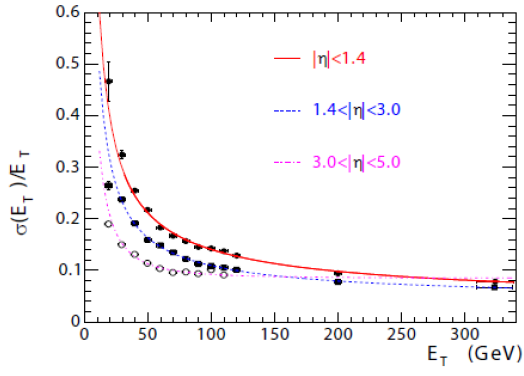
\includegraphics[width=0.5\textwidth]{HCALeRes}
      \caption{The $E_{T}$ resolution of HCAL as a function of $|\eta|$ and 
        $E_{T}$~\cite{tCmsE}.}
      \label{HCALeRes}
    \end{figure}
    
    In addition to HB and HE, HCAL has two additional calorimeters.
    Because the space between ECAL and the magnet is restricted to 1.18 m, an
    	outer hadronic calorimeter section (HO) is placed beyond the magnet
    	in the region $|\eta|<1.3$ \cite{tCmsE}.
    The main function of HO is to collect energy from the highest energy hadrons
    	before they reach the muon system.
    HO is not used in this analysis, but does contribute to the material budget. 
    To increase the total calorimetric coverage, HCAL also has a quartz fiber 
    	calorimeter (HF) in the forward region, $3 < |\eta| < 5$.
    For the majority of HF's 13 $\eta$ rings the $\eta-\phi$ segmentation is 
    	$0.175\times0.175$.
    In the lowest $|\eta|$ ring the segmentation is $0.111\times0.175$ in 
    	$\eta-\phi$.
    In the highest two $|\eta|$ rings the segmentation in $\phi$ is 0.349, with an
    	$\eta$ segmentation of 0.175 in the outer and 0.300 in the innermost 
    	ring. 
    The longitudinal direction is effectively segmented by using both short and
    	long fibers.
    The energy deposited deeper than 22cm is measured in both the short
    	and long fibers, where as the long fibers are present throughout.
    This allows electromagnetic showers to be distinguished from purely hadronic 
    	showers \cite{tCmsE}.

    The energy resolution for HF can be seen in Figure~\ref{HCALeRes}.  
    As with the ECAL, the fractional resolution increases with energy. 
    This is dues to the random nature of shower development. 
    At larger energies, the fluctuations in the shower of particles collected 
      in the calorimeter tend to average out.
    
  \section{ZDC \label{sec:zdcDet}} 
    Beyond HF, the Zero Degree Calorimeters (ZDCs) covers the very forward 
      rapidity region.
    The ZDCs sit between the beam pipes on either side of the interaction point 
      covering the area around $\theta = 0$, $|\eta| > 8.3$.
    In heavy ion collisions the ZDC has the ability to measure neutral particles 
    	that do not participate in the collision \cite{tCmsE}.
    This detector plays an important role in the analysis described in this
      thesis by measuring energy due to neutrons produced by photon-induced 
      nuclear break.
    These measurements are used to identify events with asymmetric neutron 
      emission, reducing the contribution to the sample by peripheral heavy-idon

    The ZDC has a total of 18 channels.
        Half of these 18 channels are on either side of the interaction point.
    The 9 channels on the side of CMS that correspond to positive $\eta$
      are denoted ZDC$^{+}$, where as the 9 channels on the negative side are
      denoted ZDC$^{-}$.
    The 9 channels on each side are further sub-divided into an electro-magnetic  
      (EM) section and a hadronic (HAD) section.
    The EM section is positioned in front of the HAD section with respect to the 
      interaction point and is segmented transverse to the beam direction.
    The 5 EM sections are positioned in front to absorb the energy from 
      electro-magnetically induced showers, which develop over a shorter distance 
      than hadronically induced showers.
    The transverse segmentation allows for a measurement of the transverse shower
      width and the size of the beam spot at the ZDC.
    The HAD section is segmented in the direction of the beam and consists of 4
      channels.
    The longitudinal segmentation allows for absorption of the full extended 
      hadronic shower and the ability to measure the longitudinal shower shape.
    
    Each of the 18 channels contains a tungsten target and quartz fibers.
    The dense tungsten target is used to initiate the shower.
    The quartz fibers shine Cerenkov light as the high momentum charged particles
      from the shower pass through it. 
    the light from the quartz fibers is channeled to photo-multiplier tubes, one 
      for each ZDC channel. 
    Through a cascade of photon induced electrical discharges, the photo-multiplier
      converts the Cerenkov light to an electrical pulse. 
    
    This electrical pulse travels $\sim$ 200 m down a coaxial cable from the LHC
      tunnel to the counting house in the CMS service cavern. 
    There the electrical pulse is digitized by the Charge Integrator and Encoder 
      (QIE).
    The QIE integrates the current each 25 ns.
    The charge is then mapped logarithmically to the 128 bits. 
    This bit is sent across a small fiber optic cable to the HTR firmware card.
    Here each 25 ns signal is stored in a 250 ns buffer, and the timing is synchronize
      with the rest of the detector to ensure the ZDC signal arrives at the central
      data acquisition system at the same time as the other sub detectors from the 
      same collision. 
    
  \section{Muons}
    The muon system resides just outside of the superconducting magnet.
    It consists of three complementary systems: drift tube (DT) chambers in the
      barrel, cathode strip chambers (CSC) in the endcaps, and resistive 
      plate chambers (RPC) in both the barrel and endcap regions \cite{tCmsE}.
    Each of these gaseous detectors function in the same way.
    As the muon penetrates the gas volume electrons are knocked off of the 
      gas atoms and these electrons are collected in the positively charged
      anode, whereas the ionized gas moves to the cathode. 
    The DTs in the barrel and the CSCs in the endcap have better spatial 
      precision relative to the RPCs, which are quicker and have more
      precise timing. 
    The combination of the DTs and RPCs in the barrel and the CSCs and RPCs 
      in the endcap allow for fast triggering and muon identification during
      data reconstruction. 
    \begin{figure}[!Hhbt]
      \centering
      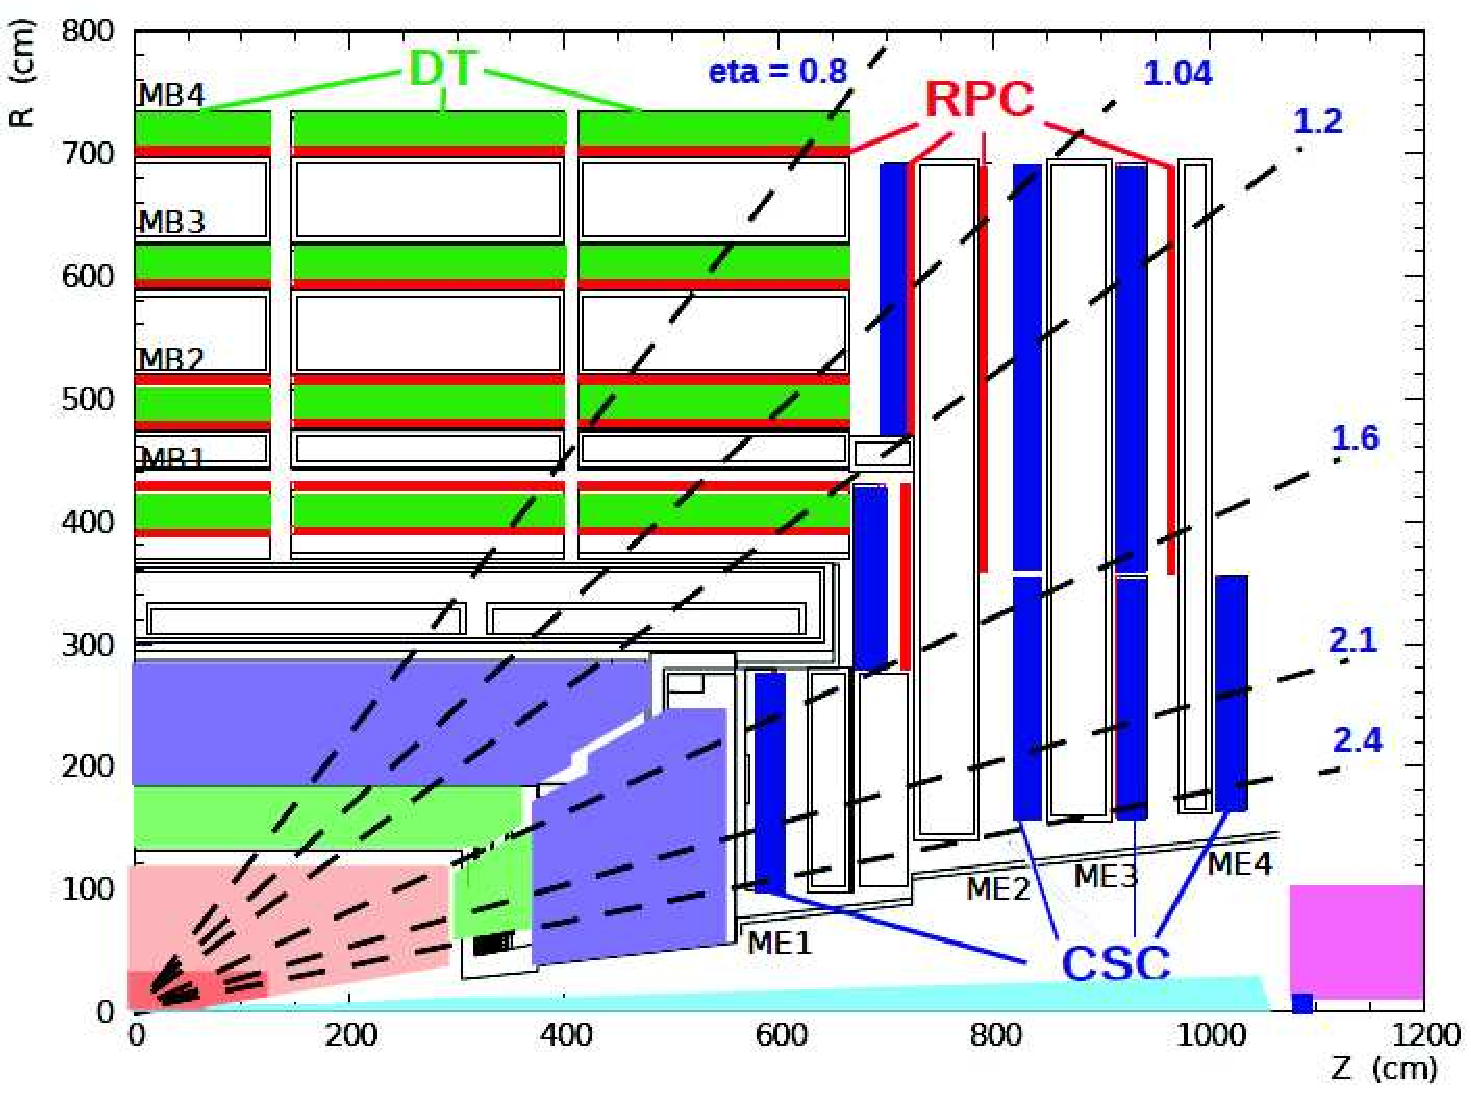
\includegraphics[width=.65\textwidth]{muonSys}
      \caption{ The CMS muon system showing the four DT stations in 
        the barrel (MB1-MB4), the four CSC stations in the endcap (ME1-ME4), 
        and the RPC stations.}
      \label{fig:muonSys}
    \end{figure}

    As seen in Fig.~\ref{fig:muonSys}, the DTs reside only in the barrel, 
      covering the region $|\eta|$ < 1.2.
    Consisting of a total of 172,000 cells, the DT cells are collected into
      250 chambers. 
    The DT chambers are in interwoven into the magnet field return yoke and are
      labeled by 5 segmentations in $z$, YB-2 to YB+2.
    Each $z$ segment is divided into 12 $\phi$ segments labeled 1 at $\phi$ = 0
      and going to 12 rotating in positive $\phi$ with segments 4 and 10 
      contain 2 chambers.
   The segmentation in $r$ is divided into four parts, MB1-MB4.
   Fig.~\ref{fig:dtSchem} shows how each chamber is made of three super layers.
   Super layers SL $\Phi_{1}$ and SL $\Phi_{2}$ measure $(r,\phi)$, whereas 
    SL $\Theta$ measures $z$.
    \begin{figure*}[!Hhbt]
      \centering
      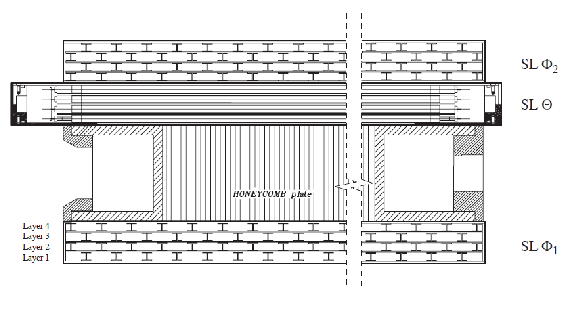
\includegraphics[width=.65\textwidth]{dtStruct} \\
      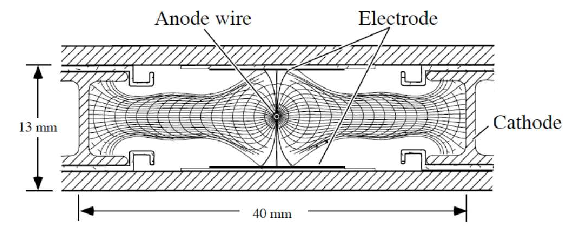
\includegraphics[width=.65\textwidth]{dtCell}
      \caption{Schematic of the DT chambers and an individual DT cell.}
      \label{fig:dtSchem}
    \end{figure*}

    The RPCs complement the DTs in the barrel and the CSCs in the endcap 
      primarily for the purpose of triggering.
    Throughout the barrel and endcap there are a total of 1020 RPC modules, 480
      in the barrel and 540 in the endcap.
    Denoted by the red lines in Fig.~\ref{fig:muonSys}, the RPCs are mounted on
      both sides of the DTs in the barrel for the inner most layers, MB1 and 
      MB2.
    For the outer two layers of the barrel, MB3 and MB4, a single layer of RPCs
      is mounted on the inner side of the DTs.
    Each corresponding DT segment has two RPCs modules, expect in MB2 where 
      some segments contain 3 RPC modules. 
    The outer ring of the muon endcap are instrumented with RPCs covering up to
      $|\eta|$ = 1.6.
    \begin{figure}[!Hhbt]
      \centering
      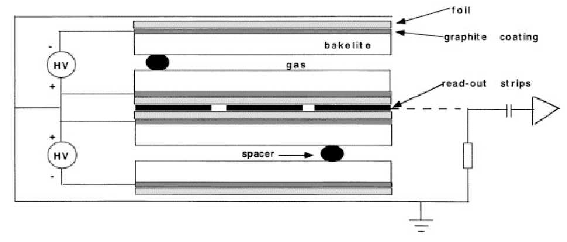
\includegraphics[width=.65\textwidth]{rpcCell}
      \caption{Schematic of a RPC cell.}
      \label{fig:rpcSchem}
    \end{figure}
 
    There is a total of 468 CSC modules in the muon system endcap. 
    For the sectors in $z$, ME2, ME3, and ME4 in the endcap, the modules in 
      the ring closest to the beam are covering 20$^{\circ}$ in $\phi$.
    The modules in ME1 and the modules in beyond in the inner ring in
      ME2 and ME3 have a 10$^{\circ} \phi$ segmentation.
    The 2 million wires of the CSCs are grouped into 400,000 channels and are
      powered with 9000 high voltage supplies. 
    The resolution of the CSCs in on the order of 1mm for position measurements 
      in the plane perpendicular to the beam and is 99\% efficient for muons
      that pass through all four sectors, ME1, ME2, ME3, and ME4.
    Because of the relatively low momentum of the muons originating from \JPsi{}
      in UPC events, the muons in the analysis discussed in this thesis are all
      in the range $1.6 < |\eta| < 2.4$ and rely on the CSCs for triggering. 
    \begin{figure}[!Hhbt]
      \centering
      $ \begin{array}{cc}
        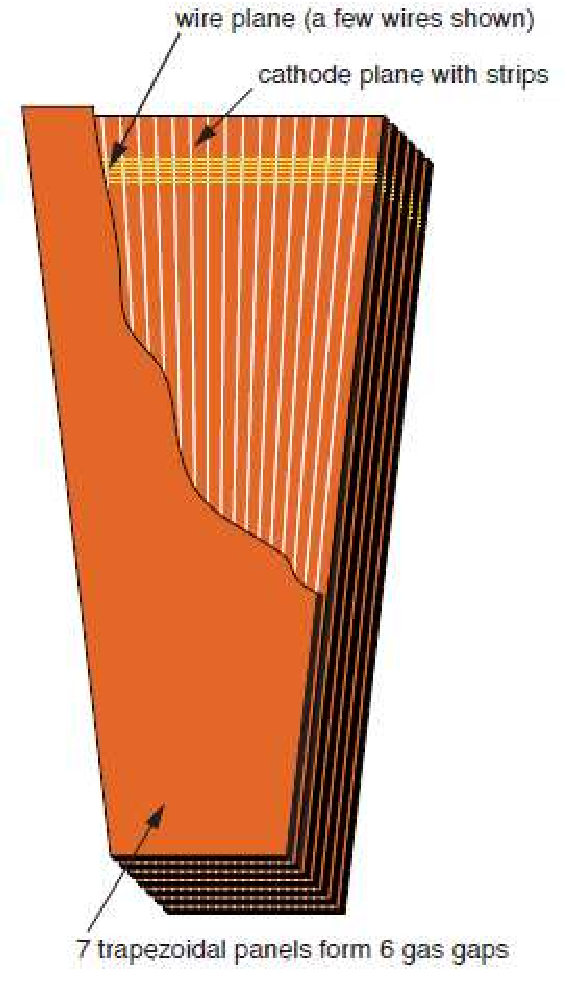
\includegraphics[width=.35\textwidth]{cscStruct} &
        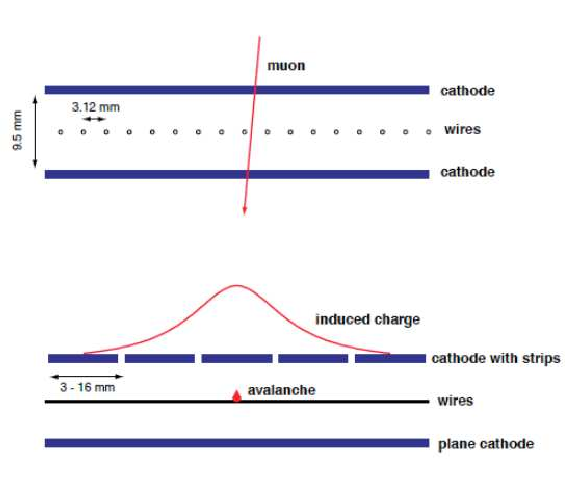
\includegraphics[width=.65\textwidth]{cscCell}
      \end{array} $
      \caption{Schematic of the CSC chambers and an individual CSC cell.}
      \label{fig:cscSchem}
    \end{figure}

    The primary function of the muon systems are to allow for triggering on and
      identification of muons.
    The tracker is still the primary instrument for measuring the muons. 
    Fig.~\ref{fig:muonRes} shows the resolution of reconstructed muons with 
      the tracker only is only improved upon for muons with momenta above 
      100 GeV. 
    For UPC \JPsi{}~events, where muons momenta are between 1-2 GeV, the muon
      system does not provide any advantage in terms of improved resolution.
    The muon system is however important in distiguishing which tracks are 
      due to muons as opposed to other charged particles.
    Because of their increase mass relative to electrons, muons emit less 
      bremsstralung, or breaking radiation, as it penetrates the inner layers
      of the CMS on its way to the muon systems.
    Fig.~\ref{fig:matThick} shows the amount of material traversed by particles
      traveling through CMS as a function of $|\eta|$.
    The total of nearly 10 interaction lengths between the interaction point 
      and the muon chambers ensures that hadrons like charged poins, which
      nearly exclusively decay to muons, are collected in the calorimeters 
      before converting to muons. 
    By eliminating backgrounds from both electrons and hadrons, the CMS muons 
      system allows for identification of muons for both triggering and 
      reconstruction.
    \begin{figure}[!Hhbt]
      \centering
      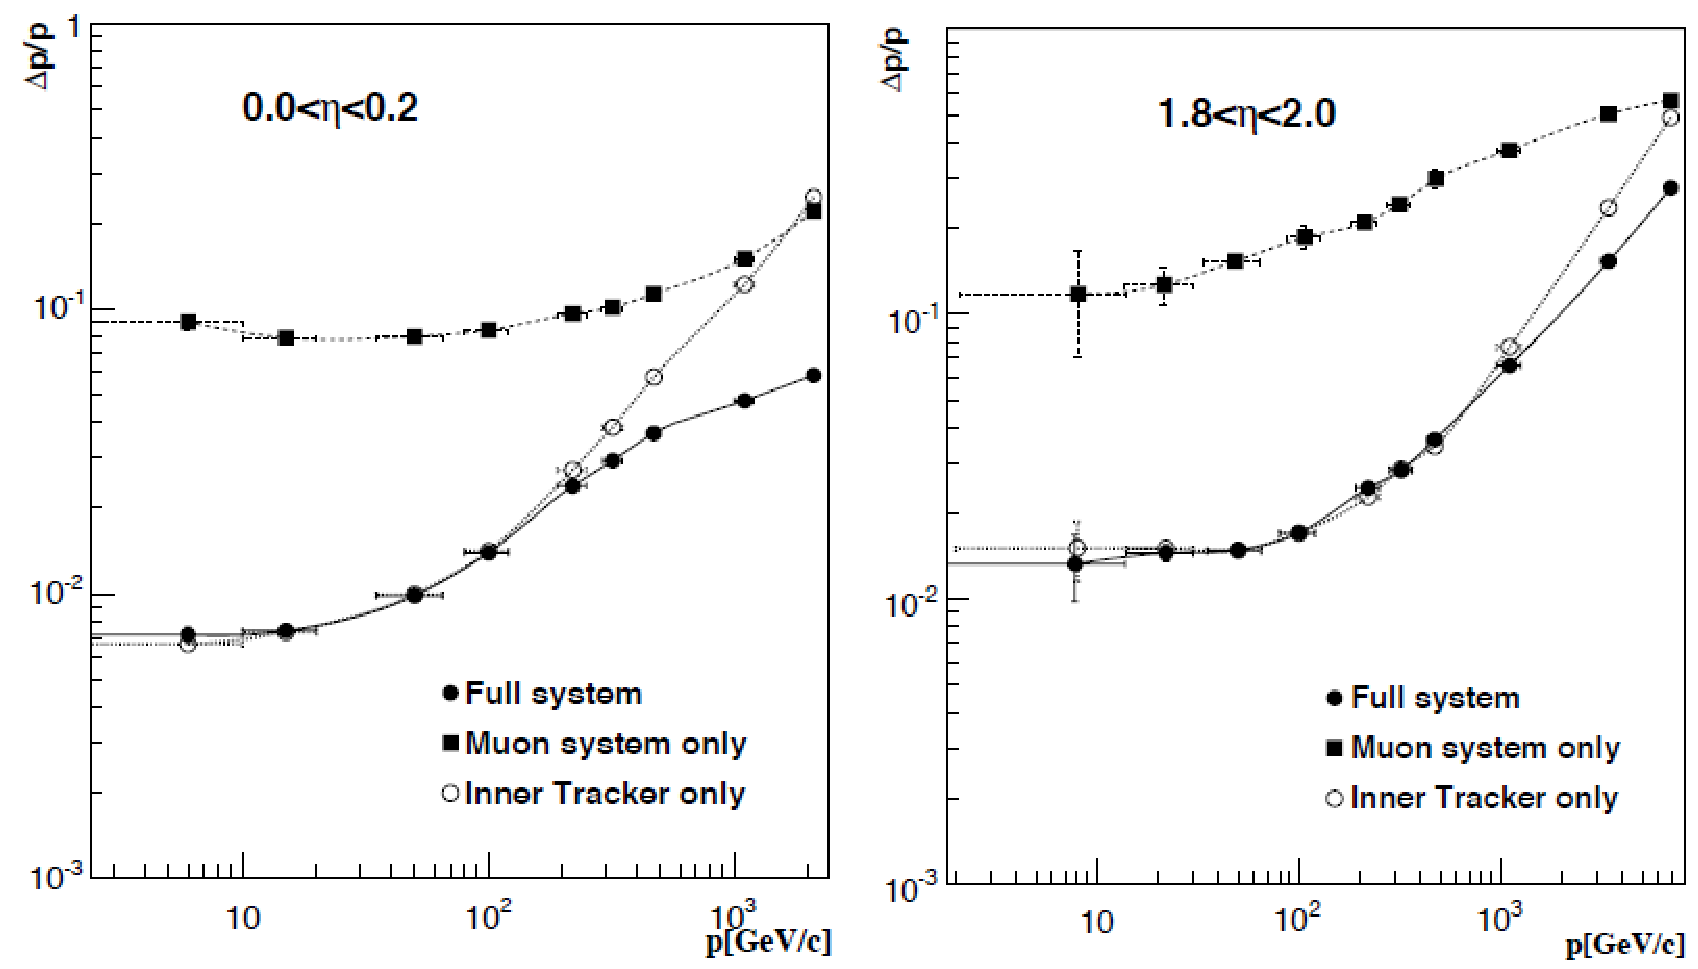
\includegraphics[width=.65\textwidth]{muonRes}
      \caption{ The momentum resolution of the muon system using only the 
        tracker and the whole muon system in the barrel (left) and end cap 
        (right).}
      \label{fig:muonRes}
    \end{figure}

    The low-momentum nature of UPC physics creates complications due to the 
      large amount of material between the interaction point and the muon 
      systems.
    About 3 GeV of momentum is needed to reach the first layers of the muon 
      system.
    In the rest frame of the \JPsi{}, the \JPsi{} equally shares its rest mass with 
      its decay products creating 2 muons with momenta of about 1.5 GeV.
    For these daughter muons to reach the muon system, their parent \JPsi{} must
      be pushed to higher momentum by the initial particles which created the
      \JPsi{}.
    For this reason, muons from UPC \JPsi{}s are only detected at higher 
      $\eta$ values.
    Understanding this momentum restriction of the muon system was a major 
      focus of the analysis discussed in this thesis with details described in 
      Section.~\ref{sec:effDet}.
    \begin{figure}[!Hhbt]
      \centering
      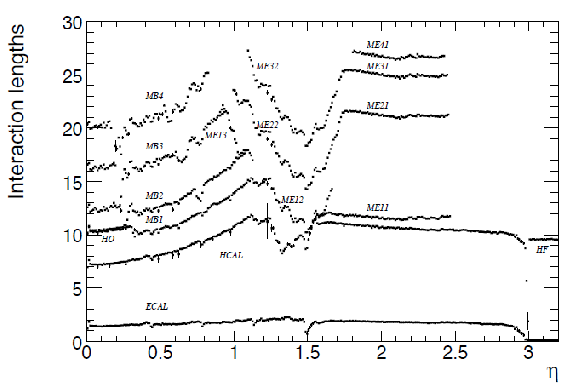
\includegraphics{materialThickness}
      \caption{The amount of material in CMS as a function of $\eta$ in 
        number of interaction lengths.}
      \label{fig:matThick}
    \end{figure}
 
  \section{Trigger}
    The CMS trigger is two tiered. 
    The L1 trigger is the lower level hardware based system. 
    The High Level Trigger (HLT) is a software base and runs on a computer farm
      located at point 5.

    The purpose of the L1 trigger is to make quick decisions about which events
      will be kept temporarily for further processing.
    The L1 trigger is used to identify events where the tracker should be read
      out.
    Only the calorimeters and the muon system are used in the L1 trigger.
    Each of the sub-detectors has its triggering hardware.
    The output from the sub-detectors is synchronized to ensure that the signal
      from each of the sub-detectors comes from the same collision. 
    The global trigger hardware then makes the final decision to initiate the 
      HLT and to read out the tracker. 

    If an event passes the L1 trigger, the data from all the sub-detectors,
      including the tracker are sent to the HLT computing farm. 
    At this level the raw data from all the sub-detectors is unpacked and 
      combined.
    The information from the calorimeters, muon system, and tracker can all 
      be used to reconstruct basic physic objects in the HLT farm. 
    For example, tracks can be associated with either ECAL energy clusters to 
      form electron candidates, tracks can be combined with hits in the muon
      system to create muon candidates.
    At the HLT, the whole detector is used to select events.
    The raw data from the events that survive the HLT are recorded permanently,
      those that do not are lost forever. 

    The HLT farm must always be ready to accept events from the L1 trigger.
    For this reason, the amount of computing time each HLT trigger path uses
      must be balanced.
    For more rare L1 triggers, which will occur at a lower rate, more 
      complex reconstruction software can be used.
    Conversely, simpler, faster, methods must be used for more common high
      rate triggers. 
    Because of this time constraint in the HLT farm, the reconstruction 
      algorithms used for triggering tended to differ from the final 
      reconstruction algorithms.
    In the HLT these algorithms are optimized for quickness, whereas the final 
      reconstruction is optimized for precision and accuracy.
    By having the ability to spend different amounts of computing time on 
      different L1 triggered events, the complexity of the event selection 
      offered by the HLT is heightened. 

    The two tiered triggering system creates very low dead times while 
      maintaining purity and selectivity.
    During data taking the L1 trigger is continuously monitoring, and the HLT
      allows for sophisticated event selection.
    The wide gamete of physics topics that are pursued by the CMS collaboration
      are a testament to the effectiveness and versatility of the CMS two 
      tiered triggering system.
    In Chapter~\ref{ch:triggChp}, the development of L1 triggers and HLT paths 
      for selecting UPC evens is discussed. 
